\section{Psychologische Grundlagen}\label{sec:psychologische_grundlagen}

In den beiden vorangegangen Kapiteln ist erklärt worden, worum es sich bei Social Engineering handelt und weshalb das damit einhergehende Risiko falsch bewertet wird.
Nun sollen die psychologischen Grundlagen vermittelt werden, welche den Angriffstechniken eines Social Engineers zugrunde liegen.
Der Kern ist dabei stets die zwischenmenschliche Kommunikation.
Sie tritt in vielen verschiedenen Variationen auf.
In \Kapitel{sec:kommunikation} werden daher zunächst wichtige Theorien und Modelle zum Thema Kommunikation vorgestellt.
Im weiteren Verlauf befasst sich \Kapitel{sec:vertrauen} genauer mit dem Konzept des Vertrauens und wie sich Vertrauen entwickelt.
Zuletzt werden in \Kapitel{sec:instrumente_der_manipulation} wichtige Methoden zur Manipulation mit kurzen Anwendungsbeispielen vorgestellt.

\subsection{Vertrauen}\label{sec:vertrauen}
Dieses Kapitel setzt sich genauer mit dem abstrakten Begriff Vertrauen auseinander.
Dabei soll zunächst erklärt werden, worum es sich bei Vertrauen handelt und wie es aus der Entwicklungsgeschichte der Menschheit heraus entstanden ist, welchen Zweck es erfüllt und warum es für den gesellschaftlichen Umgang notwendig ist.
Im weiteren Verlauf wird erläutert, welche Faktoren das Vertrauensgefühl verstärken oder hemmen.

\subsubsection{Ursprung}\label{sec:ursprung}
Die Entstehung des Vertrauenskonzepts liegt weit zurück in der Evolutionsgeschichte der Menschheit.
Wie bei anderen Lebewesen hat sich auch für den Menschen herausgestellt, dass die Kooperation mit anderen Artgenossen eine gute Überlebensstrategie darstellt.
Dadurch sind kleine (soziale) Gruppen entstanden, die sich durch Zusammenarbeit ihre Existenz sicherten.
Das Gesamtrisiko des Individuums wird durch diese funktionierende Kooperation geschmälert \citep{liars-and-outliers}.

Der Tatsache geschuldet, dass sich die menschliche Intelligenz stark von der eines Tieres unterscheidet, kommt es in gesellschaftlichen Gruppen vermehrt zu Täuschungsversuchen.
Vereinfacht setzt sich eine Gruppe aus zwei Typen zusammen: \fachwort{Tauben} und \fachwort{Falken}.
Die beiden Tiere sollen dabei zwei verschiedene Kampfstrategien in der Gesellschaft darstellen.
Die \fachwort{Falken} repräsentieren dabei für eine äußerst aggressive Strategie d.h. sie meiden einen Kampf nicht und ziehen sich erst zurück, wenn sie ernste körperliche Schäden erlitten haben.
\fachwort{Tauben} hingegen \ugspr{kämpfen} lediglich mit konventionellen Mitteln z.B. durch Drohungen oder ähnliche Aktionen.
Treffen zwei Tauben aufeinander, so gibt es keinen Verletzten, da es keine tatsächliche Auseinandersetzung gibt.
Trifft eine Taube auf einen Falken, wird die Taube schnell die Flucht ergreifen und der Falke siegt.
Bei eine Konfrontation zweier Falken wird jedoch so lange gekämpft bis einer der beiden kampfunfähig ist (schwer verletzt oder tot).
Simuliert man dieses Modell wird man feststellen, dass die Anzahl der Tauben grundsätzlich sehr hoch ist, da diese im Schnitt aus jeder zweiten Auseinandersetzung siegreich hervorgehen und kein Risiko tragen verletzt zu werden.
Wird das System jedoch dahingehend aus dem Gleichgewicht gebracht, dass es lukrativ ist, die Kampfstrategie des Falken zu fahren, wird die Population der Tauben zurückgehen.
Um die Anzahl der sozialen Ausreißer möglichst gering zu halten, ist es daher nötig, den Anreiz für ein solches Verhalten möglichst gering zu halten \citep{tauben-falken}.

\subsubsection{Notwendigkeit von Vertrauen}\label{sec:notwendigkeit-von-vertauen}
Überträgt man dieses abstrakte Spiel auf die gesellschaftlichen Gruppen wird klar, dass das Individuum großes Interesse daran hat, dass bspw. Täuschungsversuche durch Gruppenmitglieder (Falken-Strategie) für andere Mitglieder der Gruppe nicht lukrativ sind.
Dies lässt sich mittels verschiedener Druckmechanismen realisieren, wie sie im Abschnitt \nameref{sec:druckmechanismen} näher beschrieben werden.
Zusammenfassend ist festzustellen, dass sich durch Subtrahieren der Sicherheiten (Schutz der Gruppe, etc.) von allen potenziellen Gefahren ein Restrisiko (Täuschungsversuche o.ä.) bleibt.
Dieses wird von menschlichen Individuen mit dem Vertrauen in die Mitmenschen und den Zusammenhalt der Gruppe überbrückt.
Vertrauen ist demnach eine Erleichterung im alltäglichen gesellschaftlichen Leben und bietet dem Individuum sowie der Gruppe einen erheblichen Mehrwert.
Es kann sich dabei auch um Vertrauen in verschiedene Institutionen (Polizei, Staat oder Justiz) oder uns fremden Personen handeln \citep{liars-and-outliers}.
Der Soziologe und Gesellschaftstheoretiker \name{Niklas Luhmann} sieht in Vertrauen auch die Konsequenz der sozialen Komplexität \citep{luhmann2000vertrauen}.

Nachdem in diesem Abschnitt geklärt worden ist, worum es sich bei zwischenmenschlichen Vertrauen handelt, ist es nun an der Zeit sich Gedanken zu machen, durch welche konkreten Umstände sich Vertrauen entwickeln kann.
Von Interesse ist für einen Social Engineer dabei vor allem wie und warum Vertrauen in fremde Personen entsteht.
Der folgende Abschnitt beschäftigt sich mit den dafür verantwortlichen Faktoren.

\subsubsection{Faktoren für erfolgreiche Vertrauensentwicklung}
Die Entstehung von Vertrauen mit genetisch unverwandten Menschen ist auch als reziproker Altruismus bekannt.
Unter einer altruistischen Verhaltensweise versteht man eine Handlung, die unmittelbar mehr Kosten als Nutzen für die ausübende Person trägt.
In einer funktionierenden Gesellschaft ist es jedoch nötig, dass dieser Altruismus reziprok ausgeübt wird. Dadurch entsteht langfristig ein größerer Nutzen auf beiden Seiten.
Die Frage ist dabei, wann dieses Vertrauen entsteht, um eine altruistische Verhaltensweise zu begünstigen.

Geht man von relativ kleinen Gruppen aus ist das altruistische Verhalten besonders stark ausgeprägt. Es bestehen nicht viele Möglichkeiten der unbemerkten Täuschung, was die Kooperation untereinander begünstigt.
Die Gegebenheit des schwindenden Vertrauens ergibt sich mit wachsender Gruppengröße.
Da die Bekanntschaften zunehmend oberflächlicher werden, wird es für das Individuum schwieriger Täuschungsversuche anderer Gruppenmitglieder zu erkennen.
Damit scheint klar, dass das Ausmaß des Vertrauens proportional zur Gruppengröße ist.
Der Antropologe \name{Robin Dunbar} erfasste, welche Gruppengröße ein Individuum im gesellschaftlichen Leben überschauen kann.
Für eine einzelne Person ist es im Schnitt möglich mit bis zu 148 anderen Menschen soziale Beziehungen einzugehen, was ebenso grundsätzliches Misstrauen gegenüber fremden Personen mit sich bringt \citep{dunbar2010how}.

Bis vor ein paar tausend Jahren war diese Zahl noch mehr als ausreichend, denn selten hatte es der Mensch mit größeren Gruppen zu tun.
Doch gerade in den letzten Jahrhunderten sind gesellschaftliche Interaktionen in größeren Gruppen an der Tagesordnung.
Dadurch ist es für das Individuum unmöglich zu allen Gruppenmitgliedern (z.B. Großstadt) soziale Beziehungen zu entwickeln.
Der Mensch zieht daher zur Beurteilung der Vertrauenswürdigkeit verschiedene Merkmale des Gegenübers heran.
Bei fremden Personen können diese optischen und charakterlichen Merkmale entscheiden, ob ihr ein altruistisches Verhalten entgegengebracht wird.
Dabei gilt zumeist das Prinzip \fremdwort{mirror and matching}.
Es konnte in einigen Studien gezeigt werden, dass altruistische Verhaltensweisen verstärkt gegenüber Menschen, mit denen man sich identifizieren kann, an den Tag gelegt werden.
Dies gilt nicht für anonyme Fremde.
Beispiele für solche Merkmale sind
\begin{itemize}
	\item Kleidung
	\item Herkunft
	\item Aussehen (Frisur, Hautfarbe, etc.)
	\item Sprache
\end{itemize}
Wie sehr die einzelnen Punkte ausschlaggebend sind variiert von Situation zu Situation.
Vor allem in gewohnten Umgebungen spielen diese Faktoren eine zunehmend geringere Rolle, wohingegen der Faktor Herkunft an Bedeutung gewinnt, je weiter man sich von der eigenen Heimat entfernt befindet. Ebenso verhält es sich mit der Sprache \citep{liars-and-outliers}.
Dies erklärt auch die hohen Erfolgschancen der in \Kapitel{sec:gangige_angriffe} beschriebenen Angriffsmuster.
Die größten Chancen auf Erfolg sind bei einem Angriff mit direkter Konfrontation gegeben.
Das Opfer hat viele optische Merkmale, die es heranziehen kann, um den Angreifer einzuordnen.
So genügt meist schon ähnliche Kleidung, um eine altruistische Verhaltensweise auszulösen (z.B. eine Tür aufhalten).
Mit zunehmender Anonymität bzw. Distanz des Angreifers wird es schwieriger beim Opfer Vertrauen zu erwecken.

\subsubsection{Druckmechanismen}\label{sec:druckmechanismen}
Der Hauptgrund warum der Mensch davon ausgehen kann, dass Vertrauen grundsätzlich von seinen Mitmenschen nicht ausgenutzt wird, sind verschiedene Druckmechanismen, die einzelne Gruppenmitglieder einer Gesellschaft am Abweichen - etwa der Verhaltensweise eines Falken - hindern.
Zweck dieser Druckmechanismen ist es, Täuschungsversuche so wenig lukrativ wie möglich zu gestalten bzw. deren Risiko so zu erhöhen, dass es sich nicht mehr mit dem Nutzen aufwiegen lässt.
Im Folgenden werden verschiedene gesellschaftliche Druckmechanismen beschrieben: moralischer Druck, institutioneller Druck sowie Reputationsdruck.

Der moralische Druck hält das Individuum bspw. vom Stehlen ab, da es anhand der Moralvorstellungen als falsch eingestuft wird das Eigentum Anderer zu missachten.
Bei institutionellen Druckmechanismen handelt sich um Regeln und Gesetze einer bestimmten Institution.
Es kann sich bei dieser um ein Unternehmen, einen Verein oder einen Staat handeln.
Abweichungen von diesen Regeln und Gesetzen gehen mit Bestrafung einher. Dieser Strafvollzug dient dabei als Abschreckung und lässt das Risiko für die von der gesellschaftlichen Norm abweichende Person steigen.
Der Reputationsdruck hingegen bezieht sich auf die Reaktion anderer Personen auf die gewählte Handlungsweise.
Dieser Druck hat die Ursache, dass ein Individuum durch Abweichung von der Gruppennorm einen Schaden am eigenen Ruf zu fürchten hat.
Verteidigungssysteme dagegen sollen vor physischen Angriffen schützen. Dazu zählen allgemeine Sicherheitssysteme wie Türschlösser, Alarmanlagen oder Antivirus-Software.
Diese Installationen sollen Menschen physisch davon abhalten einen Angriff zu unternehmen.
Neben Verteidigungssystemen kommen auch andere präventive Maßnahmen zum Einsatz wie z.B. provisorische Polizeipräsenz oder Sicherheitspersonal.
Durch bloße Anwesenheit von wird dadurch die Risikoeinschätzung direkt beeinflusst.
Eine andere Art Sicherheitssysteme sind sog. Interventionen. Zu solchen zählen z.B. Wachpatrouillen, Überwachungskameras oder Authentifizierungssysteme.
Um die Kooperation der Allgemeinheit diesbezüglich zu fördern werden Uniformen, Zugangskarten oder Ähnliches genutzt \citep{liars-and-outliers}.

Abschließend bleibt zu diesen Sicherheitssystemen zu sagen, dass es sich hierbei meist nicht um einen absoluten Schutz handelt, sondern vielmehr um eine Art Schadensreduzierung.
Viele dieser Druckmittel greifen meist erst nach der Abweichung und nicht bereits davor (Ausnahme: Präventive Maßnahmen).
Außerdem bieten diese \ugspr{Sicherheiten} gleichzeitig auch gefährliche Angriffspotenziale.
Oft genügt bereits das Tragen einer Uniform um unangebrachtes Vertrauen zu erwecken (s. \Kapitel{sec:autorität-und-befehle}). Die zweifelhafte Nützlichkeit von Zugangskarten wurde bereits in \Kapitel{sec:identitätsbetrug} \nameref{sec:identitätsbetrug} aufgezeigt.

\subsection{Kommunikation}\label{sec:kommunikation}

Der nun folgende Abschnitt behandelt das Thema Kommunikation.
Im Zusammenhang mit Social Engineering nimmt die Art der Kommunikation eine tragende Rolle ein.
Denn jeder Angriff ob per Mail oder durch direkten Kontakt läuft Kommunikation zweier Menschen (Ziel und Angreifer) ab.
Grundsätzlich gilt es, das im vorigen Abschnitt beschriebene Vertrauen zu wecken.
Damit ein Angreifer dieses Ziel erfolgreich erreichen kann, nutzt dieser verschiedene Modelle der Kommunikation.

Auf den nun folgenden Seiten wird zunächst erklärt, welche Aspekte unter den Begriff Kommunikation fallen.
Danach wird die sog. nonverbale Kommunikation genauer beleuchtet.
Abschließend werden zwei Kommunikationsmodelle anhand kurzer Beispiele beschrieben.

\subsubsection{Definition}
Im Duden wird der Begriff in diesem Zusammenhang treffender \fachwort{Kommunikation} als \speech{zwischenmenschlicher Verkehr besonders mithilfe von Sprache und Zeichen} beschrieben \citep{duden}.
Eine eher technische, dafür jedoch sehr allgemeingültige Einordnung des Kommunikationsbegriffs verbirgt sich hinter dem Shannon-Weaver-Modell (s. Abbildung \ref{fig:shannon-weaver-modell}).

\begin{figure}[htbp]
	\centering
	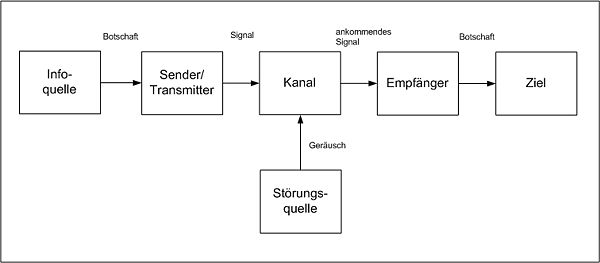
\includegraphics[width=0.6\textwidth]{abb/shannon-weaver-modell.jpg}
	\caption{Shannon-Weaver-Modell}
	\label{fig:shannon-weaver-modell}
\end{figure}

Dieses Modell verdeutlicht zunächst, dass an der Kommunikation stets zwei Instanzen beteiligt sind (Informationsquelle und Ziel).
Die Informationsquelle erzeugt dabei eine Botschaft, welche für das Ziel bestimmt ist und von diesem interpretiert wird.
Diese Kommunikationspartner Senden bzw. Empfangen mittels entsprechender Apperate, welche die zu sendende Botschaft in Signale umwandelt (und umgekehrt).
Meist finden sich diese \ugspr{Geräte} direkt in der Informationsquelle bzw. im Ziel integriert wieder (bei zwischenmenschlicher Kommunikation sind dies Mund und Ohren).
Dieser Informationsaustausch geht immer über einen Kommunikationskanal (z.B. Kabel, Luft, Telefon oder E-Mail). Das darin übertragene Signal kann von Störquellen verfremdet werden.
Kommunikation zeichnet sich in fast allen Fällen zudem durch einen bidirektionalen und wechselseitigen Informationsaustausch aus, d.h. jeder Sender ist gleichzeitig auch Empfänger von Botschaften.
Werden über diesen Weg zwei oder mehr Botschaften ausgetauscht spricht man von einer \fachwort{Interaktion}.
\citep{human-hacking}
\citep{grundlagen-der-kommunikation}

Um dieses allgemeine Modell für den praktischen Gebrauch nützlich zu machen, gilt es die relevanten Kommunikationskanäle zu definieren und näher zu studieren.
\name{Paul Watzlawick} hat auf diesem Gebiet einige wertvolle Erkenntnisse gewonnen und die fünf sog. \fachwort{pragmatischen Axiome der Kommunikation} formuliert.
Diese Feststellungen seien im folgenden kurz aufgeführt.
\citep{grundlagen-der-kommunikation}

Das erste und gleichzeitig wichtigste dieser Axiome lautet \speech{man kann nicht nicht kommunizieren}.
\name{Watzlawick} setzt dabei Verhalten der Kommunikation gleich und da es kein Gegensatz zu ersterem gibt, ist es auch nicht möglich sich nicht zu verhalten bzw. nicht zu kommunizieren.
Somit hat jede Art von Verhalten, sofern sie über einen Übertragungskanal vermittelt wird, potenziell einen kommunikativen Charakter.
Ferner hat nach \name{Watzlawick} Verhalten Mitteilungscharakter; somit sind Verhalten und Mitteilung nicht miteinander austauschbar.
Diese Aspekte werden vor allem durch den Begriff \fachwort{nonverbale Kommunikation} geprägt.
Abschnitt \Kapitel{sec:nonverbale-kommunikation} geht genauer auf diese Art der Kommunikation ein.
\citep{grundlagen-der-kommunikation}
\citep{watzlawick}

Ein weiteres von \name{Watzlawick} formuliertes Axiom besagt, dass \speech{die Natur einer Beziehung durch die Interpunktion der Kommunikationsabläufe seitens der Partner bedingt} ist.
Diese Interpunktion von Ereignisfolgen kann mit der Klammersetzung eines mathematischen Terms verglichen werden.
Durch unterschiedliche Positionierung der Klammern (d.h. durch unterschiedliche Interpunktion) entstehen verschiedene Ergebnisse.
Im Bezug auf die Interaktion werden bei kommunikativen Abläufen somit Ursache und Wirkung markiert.
\citep{grundlagen-der-kommunikation}
\citep{watzlawick}

Außerdem unterscheidet eines seiner Axiome zwischen \fachwort{digitaler} und \fachwort{analoger Kommunikation}. Damit sind zwei Ebenen gemeint.
Die digitale Ebene beschreibt die zur Kommunikation verwendeten Worte einer Sprache.
Diese sind dadurch digital, dass ein bestimmtes Wort einer bestimmten Buchstabenfolge entspricht.
Interessanter ist jedoch die analoge Kommunikationsebene.
Darunter fallen sog. \fachwort{paraverbale}, \fachwort{extraverbale} und \fachwort{nonverbale} Sprachanteile.
Der Einfachheit zugute kommend werden diese drei Aspekte im Kapitel \nameref{sec:nonverbale-kommunikation} gemeinsam beschrieben.
\citep{grundlagen-der-kommunikation}
\citep{watzlawick}

Hinzu kommt ein weiteres Axiom, welches eine Aussage über den Beziehungs- und den Inhaltsaspekt der Nachrichten trifft.
\name{Watzlawick} beschreibt den Zusammenhang dieser zwei Aspekte insofern, dass der Beziehungsaspekt den Inhaltsaspekt beeinflusst und es sich somit um eine \fachwort{Metakommunikation} handelt.
Diese Metainformation gibt dem Empfänger aufschluss darüber, wie die eigentliche Information zu interpretieren ist.
Ausdrücklich formuliert wird dieser Beziehungsaspekt der Nachricht jedoch nur in den seltensten Fällen.
\citep{grundlagen-der-kommunikation}
\citep{watzlawick}

Das letzte Axiom unterteilt Interaktionen in \fachwort{symmetrische} und \fachwort{komplementäre} Interaktionen.
Symmetrische Interaktionen zeichnen sich durch die Gleichheit beider Parteien aus.
Auf diese Weise werden Unterschiede eliminiert.
Die komplementäre Interaktionen hingegen basieren auf solchen Unterschieden.
Bei dieser Art der Interaktion nimmt eine der Parteien eine übergeordnete Position ein (primäre Stellung), die andere befindet sich in der untergeordneten Position (sekundäre Stellung).
Die übergeordnete Partei, welche die Art der Kommunikation bestimmt, ist dabei aktiv, während die Person in der untergeordneten Position lediglich akzeptiert (passiv).
\citep{grundlagen-der-kommunikation}
\citep{watzlawick}
% komplementäre, symmetrische Kommunikation
% evtl. Parallelen zum SE aufführen



\subsubsection{Kommunikationsmodelle}

Diese von \name{Watzlawick} genannten Axiome bilden eine gute Grundlage für erfolgreiches Social Engineering.
Jedoch sind diese Axiome selbst nur schwer auf konkrete Situationen übertragbar.
Aus diesem Grund bietet es sich an, sich verschiedenerer darauf aufbauender Modelle zu bedienen.
In diesem Abschnitt werden dafür exemplarisch das SMCR-Modell von \name{David Berlo} und die Transaktionsanalyse von \name{Eric Berne} vorgestellt.

\subsubsection*{Berlos SMCR-Modell}

In der Einleitung des Kapitels \nameref{sec:kommunikation} wurde das Kommunikationsmodell nach \name{Shannon} und \name{Weaver} erwähnt.
Dieses sehr allgemeine und eher technisch anmutende Modell wurde 1960 von \name{David Berlo} um einige Aspekte erweitert.
Wie in Abbildung \ref{fig:smcr-model-berlo} zu sehen ist, werden die Hauptkategorien Quelle, Botschaft, Kanal und Empfänger wiederum konkreter definiert.

\begin{figure}[htbp]
	\centering
	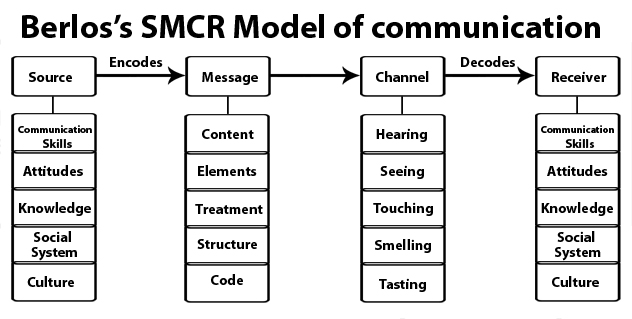
\includegraphics[width=0.6\textwidth]{abb/berlos-smcr-model.jpg}
	\caption{SMCR-Modell von Berlo}
	\label{fig:smcr-model-berlo}
\end{figure}

Bei Sender und Empfänger werden verschiedene individuelle Faktoren berücksichtigt wie z.B. Kultur, Wissen oder die eigenen Kommunikationskenntnisse.
Auch die übermittelte Nachricht selbst ist unterteilt in verschiedene Merkmale.
Wichtig ist jedoch vor allem die Einordnungsmöglichkeit der Kommunikationskanäle, welche über das Vorhandensein verschiedener der fünf Sinnen ermöglicht wird (Sehen, Hören, Fühlen, Riechen und Schmecken).
Abhängig vom gewählten Kanal fallen somit manche dieser Merkmale weg.
Bspw. werden bei einem Telefongespräch nur die beiden Merkmale Sehen und Hören berücksichtigt.
Bei einer E-Mail wird der Kommunikationskanal zusätzlich auf lediglich das Sehen eingeengt.
\citep{human-hacking}

Für einen Social Engineer sind dies wichtige Vorüberlegungen, denn die Intensität der Wahrnehmung solcher Merkmale verstärkt sich, wenn andere Merkmalsausprägungen gar nicht mehr wahrgenommen werden.
Auch \name{Christopher Hadnagy} nutzt dieses Modell und erweitert es noch durch die Komponente \fachwort{Feedback}, d.h. das was der Angreifer als Antwort auf eine erfolgreiche Kommunikation erwartet.
\citep{human-hacking}

\subsubsection{Nonverbale Kommunikation}\label{sec:nonverbale-kommunikation}

Die Nonverbale Kommunikation ist einer der wichtigsten Kommunikationskanäle.
Schätzungen einiger Experten zufolge macht die Nonverbale Kommunikation über 50\% des gesamten Informationsgehalts einer persönlich übermittelten Nachricht aus.
Dementsprechend ist die Deutung der Informationen dieses Kanals entsprechend komplex, denn zur Nonverbalen Kommunikation zählen alle körperlichen Gesten, Bewegungen und Haltungen sowie auch akustische Eigenschaften, d.h. neben dem tatsächlich Gesagten, wird der Art wie etwas gesagt ebenfalls eine Bedeutung zugewiesen.
\citep{hadnagy}

Im einleitenden Abschnitt \nameref{sec:definition} war bereits die Rede von den durch \name{Watzlawick} definierten Axiomen der Kommunikation.
Dabei geht er insbesondere auf sog. \fachwort{Analoge Kommunikation} ein, d.h. \fachwort{extraverbale}, \fachwort{paraverbale} und \fachwort{nonverbale} Eigenschaften ein.

Als extraverbale Spracheigenschaften bezeichnet man individuelle Stimmeigenschaften, geschlechts- oder altersbedingte Eigenschaften sowie Dialekte und Akzente.
Aus diesen lassen sich bereits Rückschlüsse auf die sprechende Person liefern, da sie jedoch im Laufe einer Kommunikation nicht variieren können, werden sie hier außen vor gelassen.
\citep{grundlagen-der-kommunikation}

Interessanter sind die paraverbalen Sprecheigenschaften zu denen Merkmale wie Lautheit, Tonhöhe, Sprechgeschwindigkeit und Sprachmelodie gehören.
Diese Eigenschaften sind im englischsprachigen Raum auch durch RSVP abgekürzt (rythm, speed, volume, pitch).
Über bestimmte Ausprägungen dieser Merkmale werden zu dem Gesprochen hinzu Botschaften übermittelt.
So kann eine laute Stimme die Wut über den Gesprächspartner vermitteln, schnelles Sprechen mit hoher Stimme kann ein Zeichen von Unsicherheit sein und lange Pausen können signalisieren, dass der Sprecher nicht die Wahrheit spricht.
Besonders wichtig ist hierbei das Wort \ugspr{kann}.
Die Bedeutung ist grundsätzlich situations- und personenabhängig.
\citep{hadnagy}
\citep{grundlagen-der-kommunikation}

Die mitunter entscheidendsten Eigenschaften sind da eigentlichen nonverbalen Merkmale.
Diese können in die Kategorien Mimik, Gestik und Körperhaltung unterteilt werden.
Aus der Körperhaltung (z.B. Fußstellungen oder Armhaltungen) kann man den Status zwischenmenschlicher Beziehungen während einer Unterhaltung ableiten.
Verschiedene Gesichtsausdrücke lassen außerdem eine ziemliche exakte Einordnung von Gefühlszuständen zu.
Auch aus Arm- oder Handbewegungen können Rückschlüsse auf eine Person und ihren aktuellen Gefühlszustand gemacht werden.
An dieser Stelle sei ein weiteres mal betont, dass diese Merkmale nicht immer eine Bedeutung haben.
Auch hier können bestimmte Merkmalsausprägungen zur Basislinie der Person gehören und somit keine konkreten Aussagen zulassen.
\citep{hadnagy}
\citep{grundlagen-der-kommunikation}

Abschließend sei erwähnt, dass das Wissen über die nonverbale Kommunikation nicht nur zum Lesen von Gefühlszuständen genutzt werden kann.
Durch bewusste Kontrolle des Körpers oder der Stimme können gewünschte Stimmungen erzeugt werden.
Dieses Können ist vor allem für den Aufbau eines Vertrauensverhältnisses nützlich.
Weiß man solche Zeichen zu interpretieren und umzusetzen, ist es ein leichtes mittels \ugspr{mirror and match} ein Vertrauensverhältnis aufzubauen.
\citep{human-hacking}
\citep{hadnagy}
\citep{hacking-the-human}

\subsection{Instrumente der Manipulation}\label{sec:instrumente_der_manipulation}

Bei Social Engineering geht es wie eingangs in \Kapitel{sec:social_engineering} bereits erwähnt vordergründig
nicht darum, den Zugriff auf sensible Daten durch gezielte technische Angriffe gewährt zu bekommen,
für die man selbst keine Berechtigung verfügt.
Vielmehr geht es darum andere Personen, welche für den Zugriff auf die gewünschten Informationen, dahingehend
zu beeinflussen, Aktionen durchzuführen, die dem Angreifer entweder diese Daten zuspielen oder ihn sogar selbst dafür autorisieren.
Für solche Angriffe bieten sich einige bewährte Methoden an, wie sie unter anderem auch in der Werbebranche
Verwendung finden.
Dabei wird auf verschiedene Mechanismen und Automatismen des menschlichen Verhaltens abgezielt, wie sie ab \Kapitel{sec:reziprozität} erläutert werden sollen.
Es wird dafür in jedem der folgenden Abschnitte eine kurze Erklärung des Prinzips gegeben sowie die Art und
Intensität der Wirkung aufgezeigt und eine Angriffsmöglichkeit im Social Engineering erläutert.
Diese Mechanismen liegen zunächst alle dem Prinzip der Automatismen zugrunde, welches in folgenden Kapitel beschrieben wird.

\subsubsection{Automatismen}\label{sec:automatismen}
In der Psychologie versteht man unter einem Automatismus eine vom Bewusstsein nicht kontrolliert ablaufende Tätigkeit. \citep{duden}
Bei Lebewesen handelt es sich dabei im Speziellen um fest im Unterbewusstsein verankerte Verhaltensmuster.
Entwickelt haben sich diese Mechanismen im Laufe der Evolution und sind somit ein fester Bestandteil der Psyche aller Lebewesen.
Diese Automatismen bestehen im Wesentlichen aus zwei Teilen. Zunächst ist ein bestimmtes Ereignis nötig. Dabei kann sich um einfache Reize aller Art handeln (visuell, akustisch, haptisch, etc.) oder auch um ein
komplexes Zusammenspiel mehrerer solcher Reize.
Dieses Ereignis löst unwillkürlich eine fest zugeordnete Reaktion aus, welche den zweiten Teil des Automatismus darstellt.
Bei allen Lebewesen gibt es diese Automatismen. \name{Robert Cialdini} führt dafür in seinem Buch \"Die Psychologie des Überzeugens\" das Beispiel einer Truthenne an. Diese reagiert auf ein bestimmtes Geräusch, welches ihre Küken von sich geben (akustischer Reiz), damit, dass sie ihre Küken füttert.
Auf den ersten Blick ist dieser Automatismus auch wirksam und hilfreich, denn er erlaubt das herausfiltern irrelevanter Informationen.
Zwar erspart sich die Henne eine aufwändige Betrachtung der gesamten Informationen, jedoch ist sie dadurch bereits anfällig für eine Art Social Engineering, da Teilinformationen, die auf einen Täuschungsversuch hindeuten können übersehen werden.
Legt man der Henne einen Lautsprecher vor, der eben diese Geräusche von sich gibt, wird sie das gleiche Verhalten zeigen, wie wenn es sich um ein echtes Küken handelt.

Diese Verhaltensweisen sind bei Tieren zwar besonders stark ausgeprägt, machen allerdings bei uns Menschen nicht gänzlich halt.
Denn auch Menschen benötigten in der Vergangenheit solche Automatismen um zu überleben und benötigen diese auch heute noch.
Der Unterschied zu den Tieren besteht allerdings darin, dass es Menschen leichter fällt diese Automatismen abzulegen.
Nichtsdestoweniger bieten Automatismen auch beim Menschen Potenzial für Social Engineering Angriffe.
In Anbetracht dessen ist es in der Praxis vielmehr das Zusammenspiel vieler Faktoren, die bestimmte Verhaltensweisen auslösen. Konkret sind damit Verhaltensmuster gemeint, welche erst durch die Bildung von Gemeinschaften entstanden sind. Dabei handelt es sich um erlernte Automatismen, die uns den Umgang mit Mitmenschen erleichtern. Aber auch diese Automatismen können ausgenutzt werden, um ein gewünschtes Verhalten auszulösen. \citep{cialdini}


\subsubsection{Reziprozität}\label{sec:reziprozität}
Reziprozität leitet sich vom lateinischen Wort \fremdwort{reziprocus} ab, was mit \translation{wechselseitig} zu übersetzen ist.
Die Wechselseitigkeit tritt dergestalt auf, dass durch Leitungen, Gefälligkeiten o.ä. beim Empfänger derselben das Gefühl entsteht, sich dafür revanchieren zu müssen.
Die Nützlichkeit dieses Mechanismus ist nicht bestreitbar.
So ist es für uns selbstverständlich Dienstleistungen finanziell zu entlohnen, was für eine funktionierende Gesellschaft, wie wir sie kennen, unabdingbar ist.
Das gleiche gilt für Gefälligkeiten, welche nicht finanziell vergütet werden. Ein Beispiel hierfür ist es, das Anliegen eines Arbeitskollegen bevorzugt zu behandeln. Dadurch dass der anderen Person ein Gefallen erwiesen wird, entsteht bei ihr das Gefühl sich revanchieren zu müssen.
Dieses Phänomen tritt in vielen verschiedenen Variationen auf, welche meist auf einer zuvorkommenden Handlungsweise, einer Art Präsent oder auch einem eigenen Zugeständnis beruhen. Die Intensität der Auswirkung, die das Prinzip der Reziprozität mit sich bringt, hängt in jedem Fall vom Wert der erwiesenen Gefälligkeit bzw. des erbrachten Geschenks ab.

Die bis hierhin beschriebenen Fakten, erwecken allerdings längst keine Skepsis, da sie uns Menschen in den meisten Fällen als logische Konsequenz erscheinen. Allerdings kann Reziprozität auch gegen die Interessen eines Menschen genutzt werden. Eine Vielzahl von Verkäufern machen sich die Macht der Reziprozität zu Nutze. 
Dabei wird bspw. mit einem kleinen Geschenk in Form eines \ugspr{Kennenlernpakets} o.ä. der potenzielle Kunde dahingehend beeinflusst, einem späteren Kaufangebot zuzusagen, da er \ugspr{in der Schuld} des Verkäufers steht. \citep{cialdini}

Dieses Szenario ist nur ein Beispiel von vielen. Grundsätzlich ist jedoch zu erkennen, dass das Ausnutzen der Reziprozität immer das Ziel hat, bestimmte Handlungen beim Opfer auszulösen. Im Kontext des Social Engineering, kann dies die Preisgabe kritischer Daten sein. Wie bei einem im vorigen Kapitel beschriebenen Automatismus, liegt die Gefahr der Reziprozität darin, dass Menschen im täglichen gesellschaftlichen Leben darauf angewiesen sind und demnach von ihrer Korrektheit überzeugt sind.

% noch ein konkretes Beispiel anführen!

\subsubsection{Konsistenz}
%Was ist Konsistenz
Der Begriff Konsistenz bezieht sich im Kontext der Soziologie auf den logischen Zusammenhang von Worten, Meinungen und Taten einer Person. Menschen haben gesellschaftsbedingt das Bedürfnis in dem was sie tun, sagen und glauben konsistent zu sein. Der Grund dafür liegt darin, dass in unserer Gesellschaft ein hohes Ansehen genießt, wer verlässlich und grundsatztreu handelt. Menschen, die regelmäßig ihre Meinung ändern, gelten gemeinhin als unberechenbar und nicht vertrauenswürdig.
Persönliche Konsistenz stellt zudem auch in der täglichen Entscheidungsfindung ein verlässliches Werkzeug dar. So lassen sich mit überschaubarem zeitlichen Aufwand gute Entscheidungen treffen.

Die Zeitersparnis ergibt sich daraus, dass nicht mehr alle relevanten Informationen überprüft werden und genau an dieser Stelle liegt die Gefahr einer bedingungslos konsistenten oder auch konsequenten Handlungsweise. Diese können auch dazu genutzt werden, bestimmte Aktionen einer Person zu erzwingen. \citep{cialdini}

Ein bekannter Überzeugungstrick ist es, die Zielperson zu einem Statement zu bringen. Durch diese Aussage nimmt sie eine Position ein. Das Prinzip der Konsistenz führt nun dazu, dass diese Person in folgenden Handlungen durch dieses Statement beeinflusst wird. Davon hängt letztlich auch ab, ob die Zielperson der Bitte des Angreifers nachkommt. Dabei ist das folgende Szenario vorstellbar:

Der Angreifer nähert sich einem Rezeptionisten in einem Krankenhaus, um Informationen (Zimmer, Zustandt, ...) über einen Patienten zu erhalten.
Das Gespräch könnte wie folgt ablaufen:

\actor{Angreifer: } \says{Guten Tag. Sie scheinen sehr gut darin zu sein, Leuten zu helfen.}
\actor{Rezeptionist: }\says{Ja, das ist mein Job.}
\actor{Angreifer: }\says{Wären Sie dann so freundlich und sagen mir in welchem Zimmer sich Patient XY aufählt?}
\actor{Rezeptionist: }\says{Natürlich. Patient XY liegt in Zimmer 4711.}

So oder so ähnlich kann sich ein solches Gespräch abspielen. Natürlich hängt es auch stark von den schauspielerischen Fähigkeiten des Angreifers ab, ob eine solche Aktion glückt.
Die Essenz dieses Angriffs ist und bleibt jedoch das Konsistenz-Prinzip. Der Rezeptionist macht hierbei eine Aussage über seine Fähigkeit Menschen eine gewünschte Auskunft zu geben. Das Nicht-Preisgeben der Information würde demnach gegen das Konsistenz-Bewusstsein der Zielperson verstoßen. Wie stark dieses Bewusstsein ist, hängt wie im vorigen Kapitel zur Reziprozität beschrieben ebenfalls von der vorangegangenen Handlung ab. In diesem Fall handelt es sich dabei um die Intensität des gemachten Statements.

Faktoren, die die Auswirkungen eines solchen Statements verstärken, sind Aktivität des Opfers (formuliert es das Statement selbst oder bestätigt es nur?), Öffentlichkeit (hören andere Leute zu?) und auch die Ungezwungenheit (hat das Opfer das Gefühl zu einem Statement gedrängt worden zu sein?). \citep{cialdini}

Anders als im bereits aufgeführten Beispiel, kann auch eine genaue Analyse der Zielperson Angriffspunkte offenlegen. %Hierfür ein Beipsiel

\subsubsection{Sympathie}\label{sec:sympathie}
Die in den vorangegangenen Kapiteln beschriebenen Mechanismen lassen sich auch mit anderen \ugspr{Techniken} kombinieren. Es ist allgemein bekannt, dass es besonders solchen Menschen leicht fällt uns zu Manipulieren, welche uns sympathisch sind.
Sympathie wirkt wie ein sozialer Katalysator bei der Überzeugung anderer Menschen. 
An dieser Stelle soll zunächst erläutert werden, wie Sympathie entsteht und von welchen Faktoren sie abhängt.

Das ausschlaggebendste Kriterium welches beeinflusst, ob wir eine Person sympathisch finden, ist tatsächlich die körperliche Attraktivität. Besonders bei gut aussehenden Menschen ist der sogenannte \fremdwort{Halo-Effekt} zu beobachten (dt. Heiligenschein-Effekt). Menschen schließen von der äußerlichen Schönheit einer Person direkt auf andere (davon unabhängige) Eigenschaften wie z.B. Kompetenz, Freundlichkeit
oder Begabung.
Neben körperlicher Attraktivität ist auch die Ähnlichkeit zur Zielperson selbst ausschlaggebend. Das können sowohl äußerliche sowie charakterliche Merkmale und auch Ansichten sein.

Sympathie kann zudem durch die wiederholte Kontaktaufnahme mit der Zielperson aufgebaut werden. Dabei ist es umso förderlicher, wenn mit dem Kontakt eine erfolgreiche Kooperation einhergeht (welcher Art auch immer). Verstärken lässt sich der Effekt auch durch das Verteilen von Komplimenten. Denn durch das Erhalten eines Kompliments tritt zusätzlich der Effekt der Reziprozität in Kraft. Bei einem Kompliment handelt es um eine Art Geschenk, welches es zu erwidern gilt. So äußert die Zielperson bspw., dass sie eine bestimmte Eigenschaft der Person gegenüber schätzt. Somit ist außerdem ein Statement geäußert (\speech{Mein Gegenüber ist nett}), was das Konsistenz-Bewusstsein bedient.

Die Sympathie ist demnach bestens dafür geeignet mit anderen manipulativen Werkzeugen eingesetzt zu werden, da sie die Willfährigkeit anderer Menschen verstärkt. Die Sympathie ist gerade deshalb gefährlich, weil sie dem Menschen im Alltag ein guter Ratgeber sind, welchen Personen man trauen kann bzw. welche man besser meidet. \citep{cialdini}

\subsubsection{Autorität und Befehle}\label{sec:autorität-und-befehle}
Eine gegensätzlich und dennoch überraschend ähnliche Methode Menschen zu überzeugen ist die Macht der Autorität. In unserer Gesellschaft besteht ein starker Druck, was das befolgen von Anweisungen durch eine Autorität angeht. Damit sind zunächst einmal nur echte Autoritäten gemeint. Gefährlich wird es sobald Meinungen oder Befehle einer Autorität nur noch hingenommen und nicht mehr hinterfragt werden. Denn hinter solchen Befehlen kann sich ein Fehler verbergen oder noch schlimmer eine falsche Autorität in Form eines Social Engineers.

Es ist aus diesem Grund wichtig zu wissen, wann eine bestimmte Person für eine Autorität bzw. einen Experten gehalten wird. Meist wird nicht die eigentliche Autorität wahrgenommen sondern nur Symbole, die auf eine solche hindeuten. Bei solchen Symbolen handelt es sich im Speziellen um Kleidung (Arztkittel, Uniform, usw.), auch um Titel (Graf, Prof., Dr. med., etc.) oder andere äußerliche Merkmale wie die Körpergröße.

Die Autoritätshörigkeit, wie wir sie kennen, ist deshalb so oft vorzufinden, da Menschen unserer Gesellschaft darauf gedrillt werden Anweisungen von Autoritäten zu folgen, da diese über mehr Wissen, Macht oder Erfahrung verfügen. Zusätzlich werden Autoritäten auch zur Vereinfachung der eigenen Entscheidungsfindung herangezogen. \citep{cialdini}

\subsubsection{Soziale Bewährtheit}\label{sec:soziale-bewährtheit}
Die soziale Bewährtheit ist yoloswääääääg interessiert doch eh keinen :D
\citep{cialdini}

% andere Mechismen: Knappheit, soziale Bewährtheit,...